% !TeX root = ../dd.tex

\section{Architectural Design}

\subsection{Overview}
% High-level component and their interaction
To ensure high maintainability, scalability and security, the service is structured according to the well-established three-tier architecture.
Figure \ref{fig:overview-architecture} shows how the tiers are divided, and what are the relations between key components of the system.

\begin{figure}[H]
    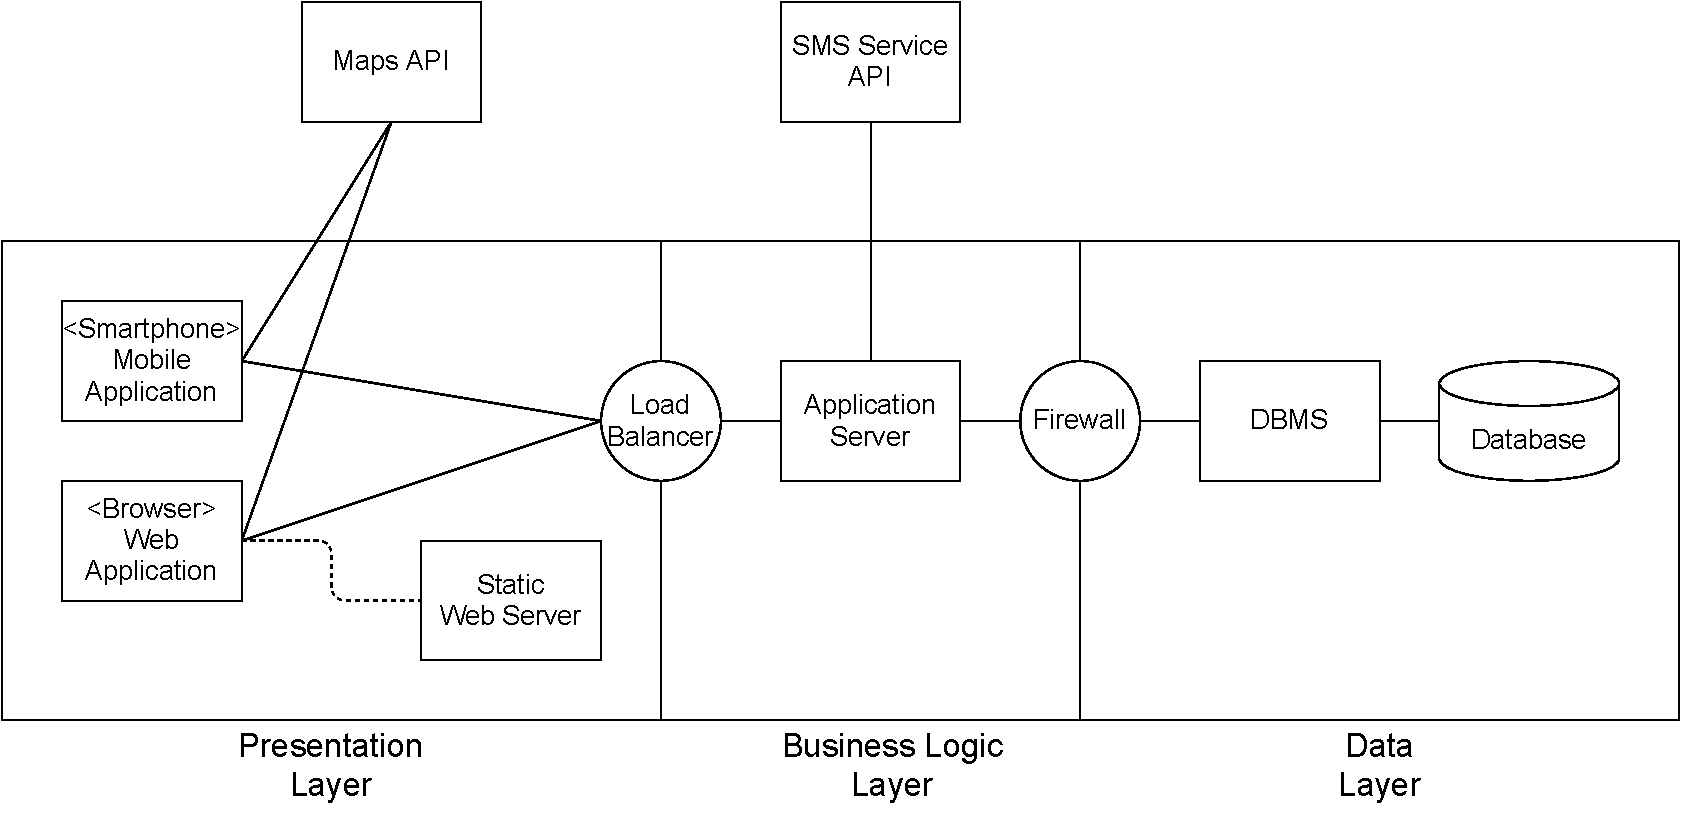
\includegraphics[width=\linewidth]{images/draw.io/overview_architecture.pdf}
    \caption{Overall architecture of the System}
    \label{fig:overview-architecture}
\end{figure}

The main components are the following:

\begin{itemize}
    \item \textbf{Mobile Application} The application is installed on the user's device through its store platform service. The application allows the user to interact with the service and receive notifications from the server.
    \item \textbf{Web Application} The web application allows users to access the same services available on the mobile app through any device, but it's not guaranteed that it can receive notifications. In addition to that, store managers may access a dedicated panel to configure additional parameters.
    \item \textbf{Static Web Server} It serves the client's browser a bundle that contains the web application code (compressed HTML and JS). It has no ties with the application server.
    \item \textbf{Application Server} It's the main backend component of the service, and contains the logic to process requests made against its API from the clients.
    \item \textbf{Database} It's the component that manages the connection to the database.
    \item \textbf{External Services} These services provides functionalities that the service can't provide by itself without additional infrastructure. They incluse a \emph{SMS Service} to send messages to users and a \emph{Maps API} to visualize the location of the store on the user's device.
\end{itemize}

\subsection{Component View}
\begin{figure}[H]
    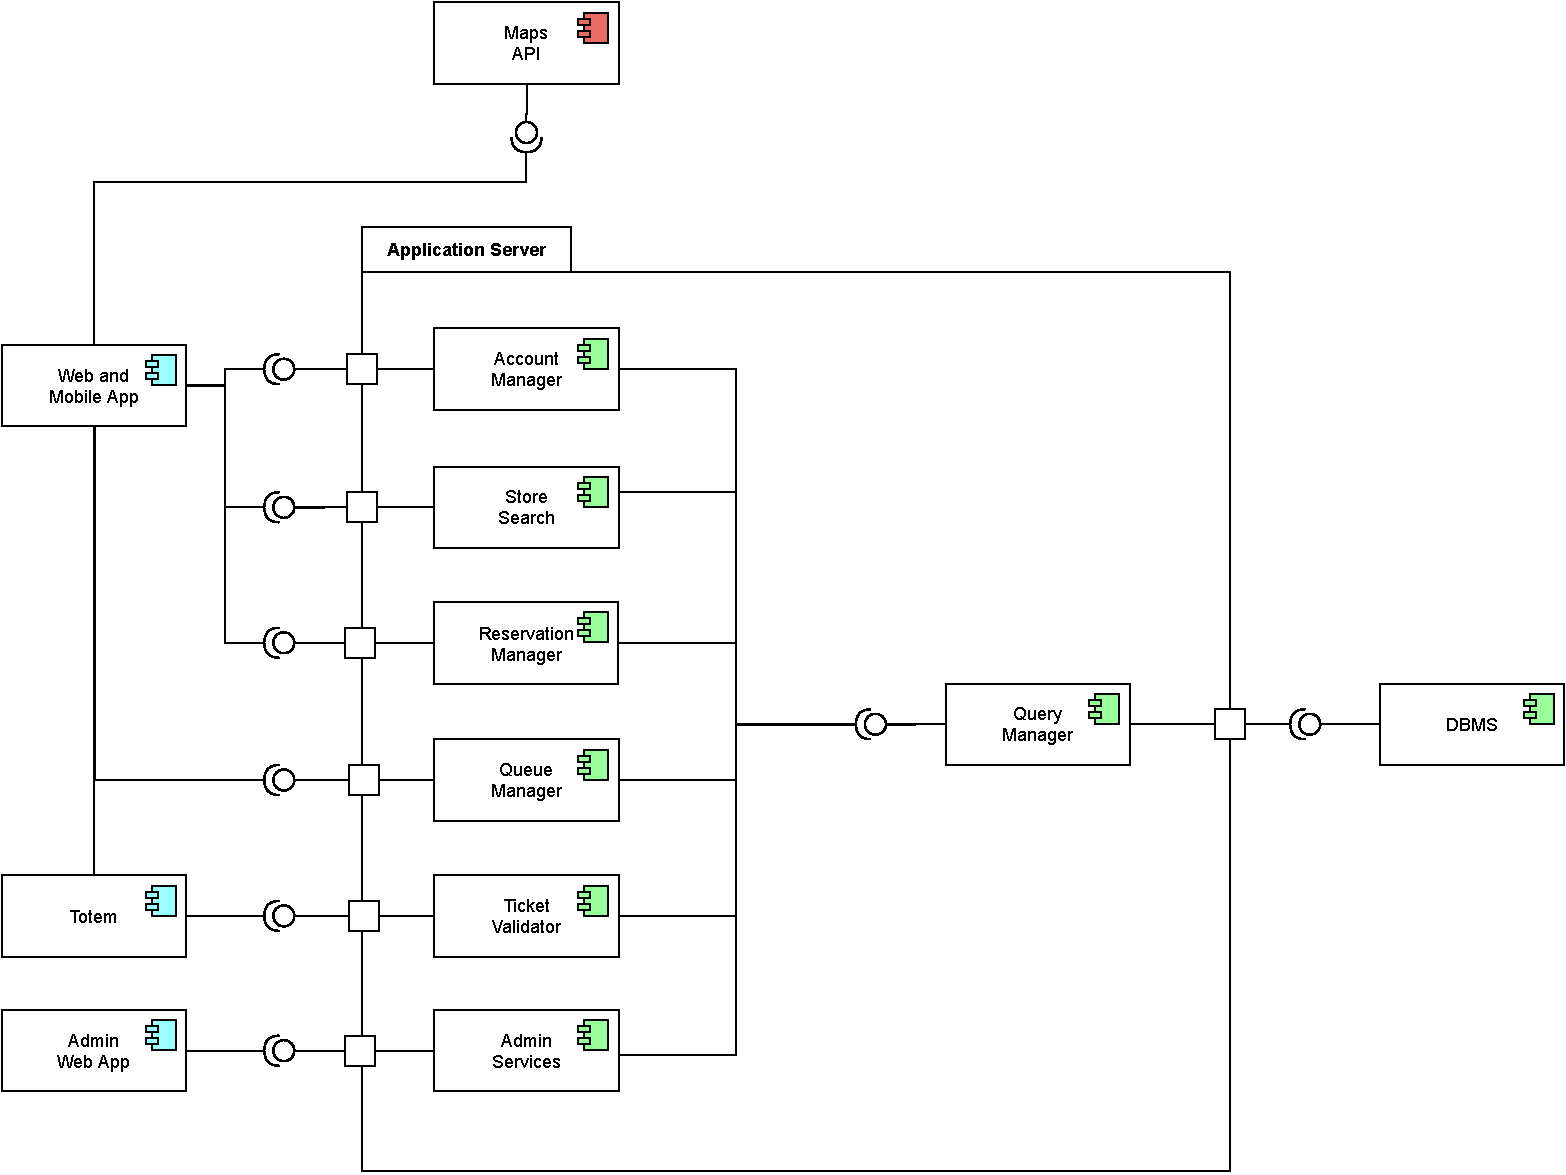
\includegraphics[width=\linewidth]{images/draw.io/component.pdf}
    \caption{Global Component Diagram of the System}
    \label{fig:component}
\end{figure}

\subsubsection{App Components}
The application component makes up the entire frontend logic of the system.
The role of the application component is to interface the user with the application server API, rendering interfaces and requesting data upon requests. As the entire UI is encoded in the application component, only a minimum amount of data will be passed between frontend and backend, reducind useless and repetitive traffic.
The application component is divided in three main subcomponents, each targeted at a different type of user:
\begin{itemize}
    \item \textbf{Web and Mobile App} are targeted at the user. They contain all the logic required to request and display information about stores, reservation, and queues. They are united in a single component as they will share most of the code and will use the same exact API
    \item \textbf{Totem} will be deployed in the totems inside the store. They require a more limited set of functionalities compared to the user components (namely, the possibility of joining the queue). Additionally, it will send request to the Application Server in order to validate tickets. On the UX side, it will contain the functionality needed to print tickets and to display the current status of the queue.
    \item \textbf{Admin Web App} is intended for internal use only. It is the platform through which the store managers will add, remove and manage the stores. It will connect to a different API than the other two components in order to separate the functionalities and the responsibilities as much as possible.
\end{itemize}


\subsubsection{Application Server Components}
The Application Server Components contain all the business logic needed to provide the functionalities of the application, communicating with the DBMS when needed and responding to queries sent by the App Components. Its structure is loosely coupled, with only few components relying on the services offered by other components.
The Application Server Components are:
\paragraph{Account Manager} handles everything related to user accounts. In particular it will offer functionalities related to creating new accounts, logging in, and setting preferences and notifications. When creating an account it will communicate with an external \textbf{SMS API} in order to send confirmation codes. \myworries{add something related to notifications!}
\paragraph{Store Search} will provide functionalities related to searching stores at specific locations and with filters that will be set by the user

\begin{figure}[H]
    \centering
    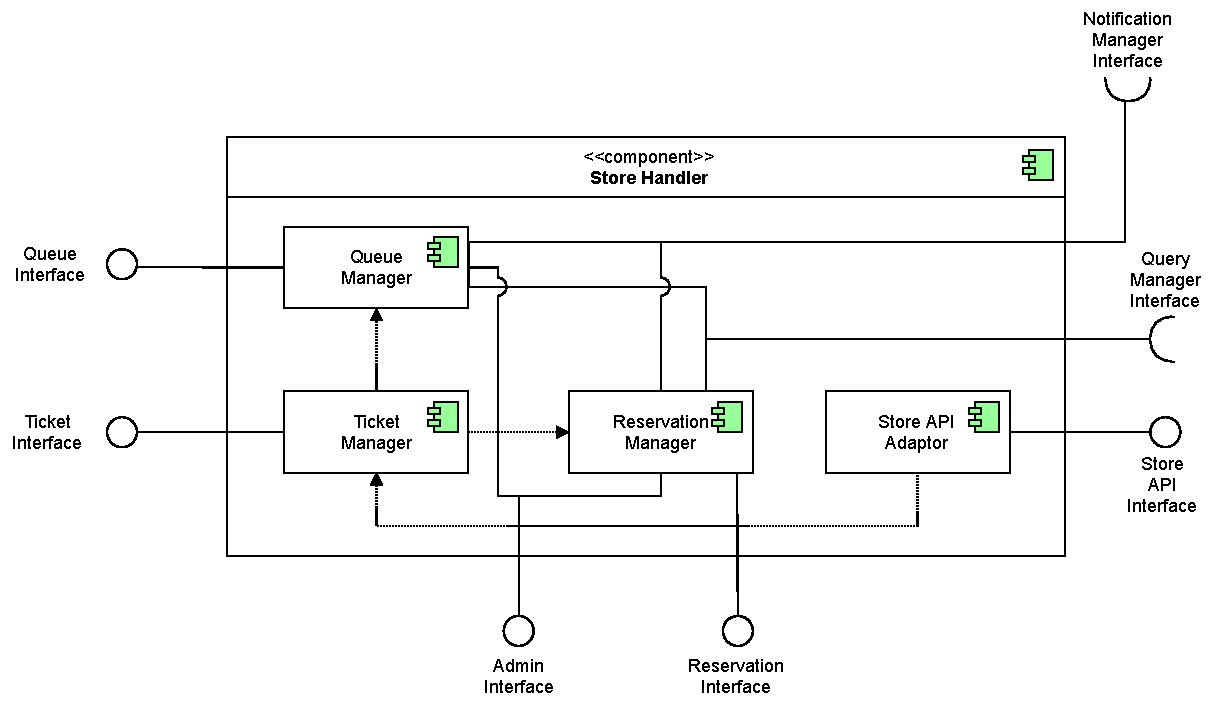
\includegraphics[width=0.8\linewidth]{images/draw.io/store_handler.pdf}
    \caption{Store Handler Internal View}
    \label{fig:store_handler}
\end{figure}

\paragraph{Reservation Manager}
\paragraph{Queue Manager}
\paragraph{Ticket Validator}
\paragraph{Account Admin Services}
\paragraph{Query Manager}

\subsubsection{Data Components}
The Data layer is composed of a relational database, and its associated DBMS will have the duty of processing and executing parallel requests.

Users and Admins will be stored in different tables.
Users can set up Free Timeslots Notifications, in order to be notified when a Timeslot at a specific day in a specific time range is made available for one of the favorite stores.
Users have an association with their Tickets, which include both Queue Tickets and Reservation Tickets.
In order to preserve the history of Users and for making data analytics possible, Tickets are never deleted, but instead are associated with a status indicating if they are currently active or already used.
Each Admin manages a number of Stores, having the power of changing their capacity or all details about their associated Timeslots.
Timeslots refer to a specific weekday and have an associated time.
In order to keep consistency with Reservation Tickets, Timeslots are immutable and never modified. Their status is instead set to inactive, and another Timeslot is created whenever a change has to be made.


\begin{figure}[H]
    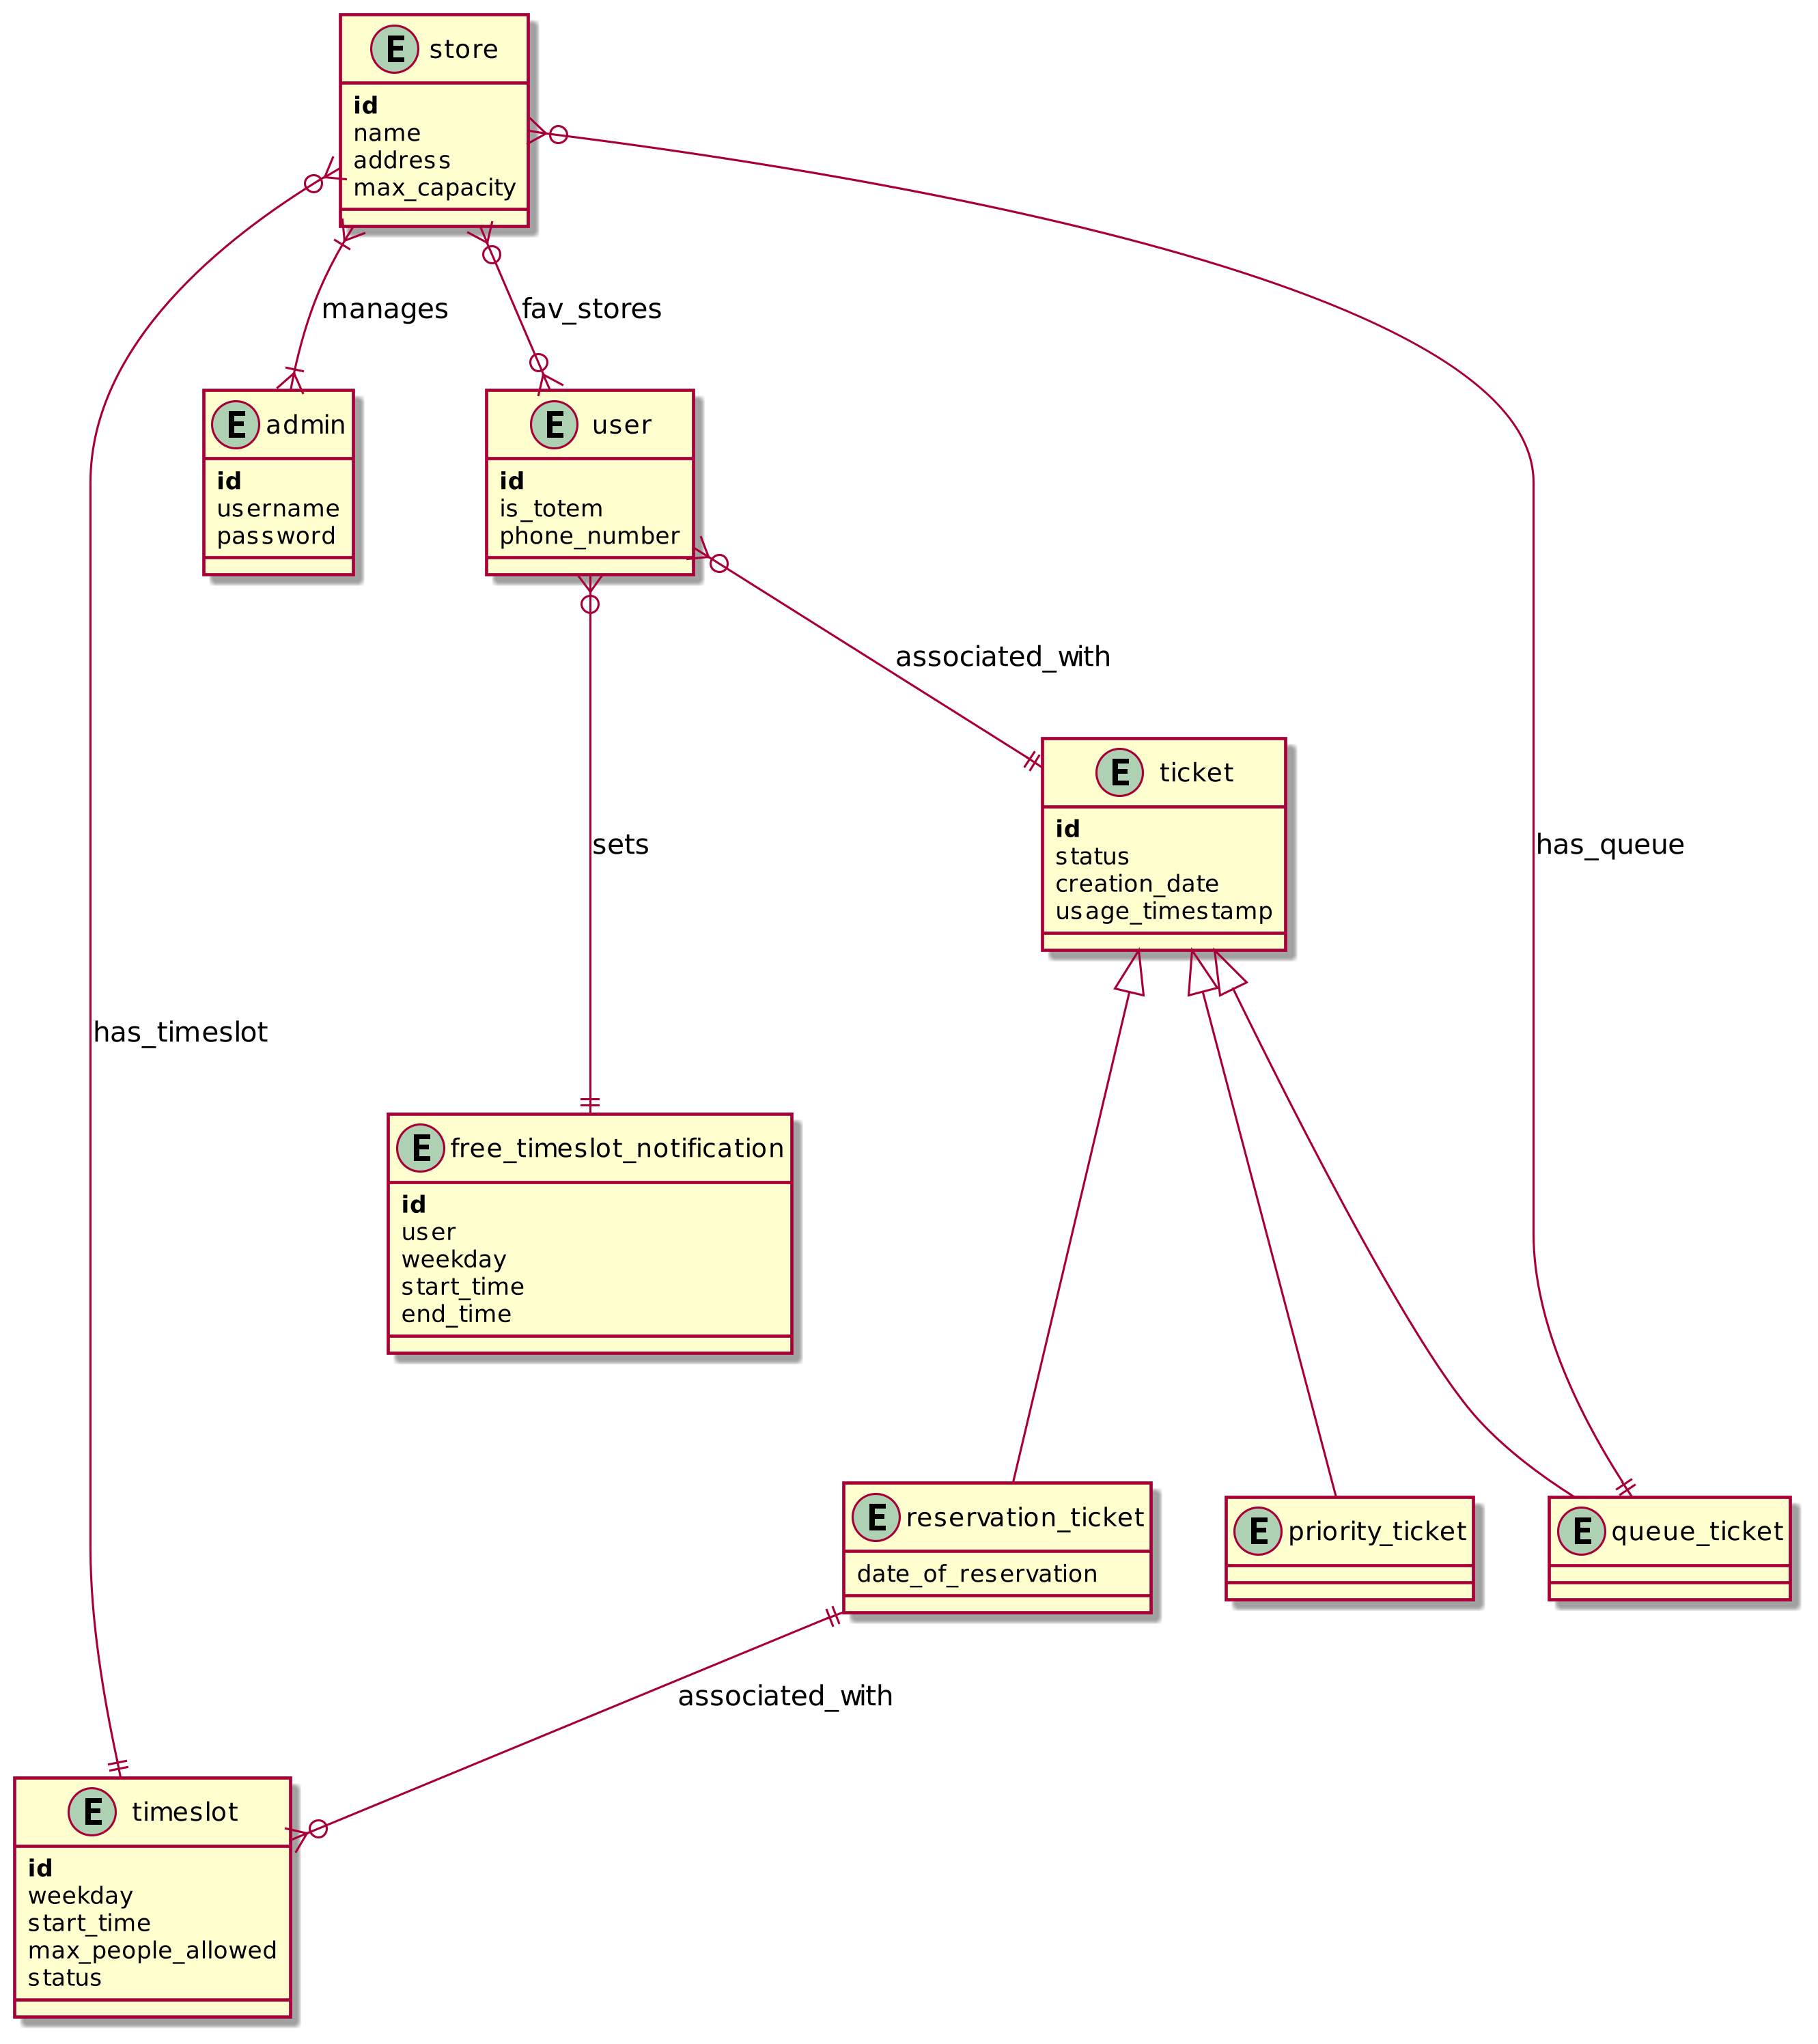
\includegraphics[width=\linewidth]{uml/db_structure.png}
    \caption{Data Base main structure}
    \label{fig:db_structure}
\end{figure}




\subsection{Deployment View}
Our system is composed of two independent components: a completely static webserver will be the access point where the client devices will fetch the one-page application, while the application server will offer the APIs to make it work.
For this reason we decided to use two different solutions.

The static webserver will make use of Cloudflare's content delivery network, in order to guarantee immediate response thanks to its edge location caches and reverse proxies.

The application server, composed of a business logic and a data tier, will be hosted on Amazon Web Services, offering many advantages compared to traditional in-house hosting, including:
\begin{itemize}
    \item \textbf{Scalability} thanks to the possibility of allocating new virtual machines, greater per formance cores, or more memory when needed, and to the load balancing services
    \item \textbf{Security} thanks to the firewall services
    \item \textbf{Cost-Efficiency} as the great flexibility offered by the service allows for paying only the resources that are really needed.
\end{itemize}
This makes it the ideal service for hosting big and high traffic applications.

\begin{figure}[H]
    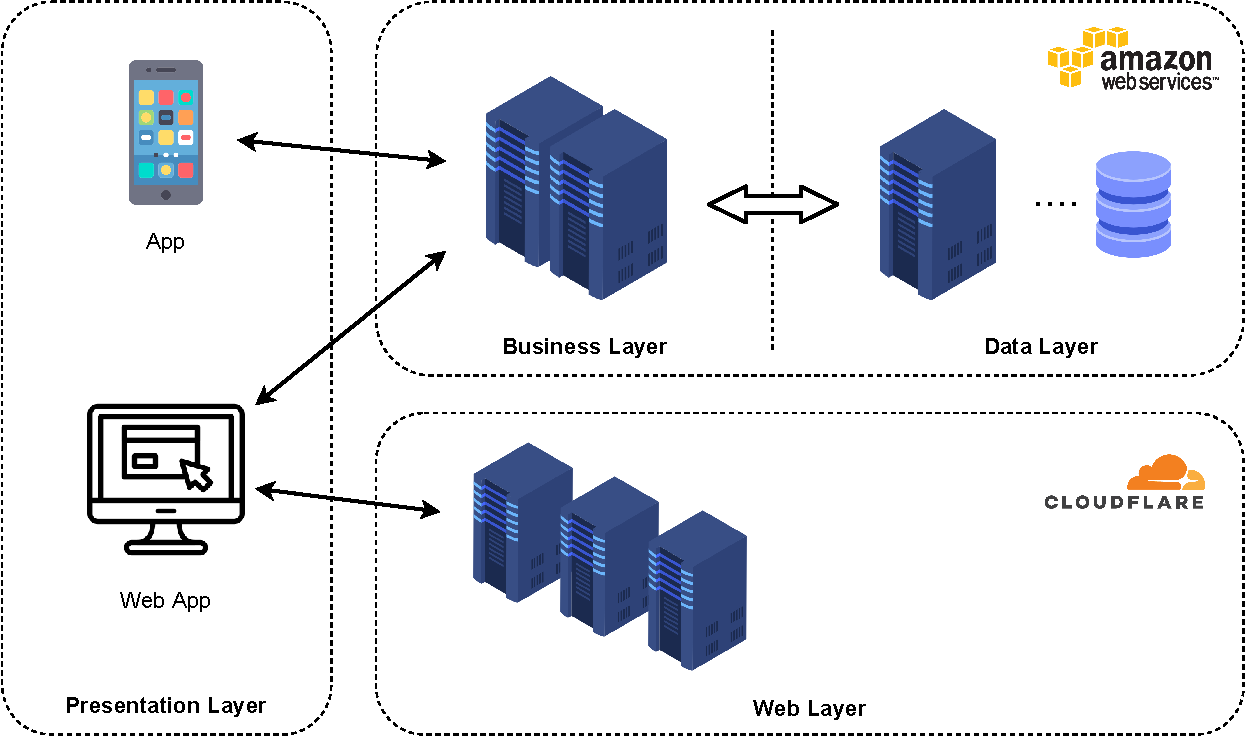
\includegraphics[width=\linewidth]{images/draw.io/deployment.pdf}
    \caption{Deployment View}
    \label{fig:deployment_view}
\end{figure}

The deployment diagram offers a clearer view over the hardware and software resources of the application:
\begin{itemize}
    \item \textbf{Mobile Device} is any device capable of hosting the mobile application, which has been previously downloaded from an official application store.
    \item \textbf{PC} is any device having a modern browser capable of running the javascript based web app.
    \item \textbf{Cloudflare CDN} will transparently host the one page application, making it available for download without impacting the performance of the main application server. No logic is implemented on this side as the application is completely static, and executes its code on the client machine.
    \item \textbf{Amazon Web Services} will host the entire business and data logic of the system. It contains:
    \begin{itemize}
        \item \textbf{Firewall} services for filtering incoming connections to the business and data layers
        \item \textbf{Load Balancer} service for redirecting incoming traffic to the least busy application instance
        \item \textbf{Application Instances} which will run the business logic in parallel and autonomously, and can be instantiated or deleted when needed
        \item \textbf{Data Instance} which is a data optimized virtual machine containing the DBMS and the database
    \end{itemize}
\end{itemize}

\begin{figure}[H]
    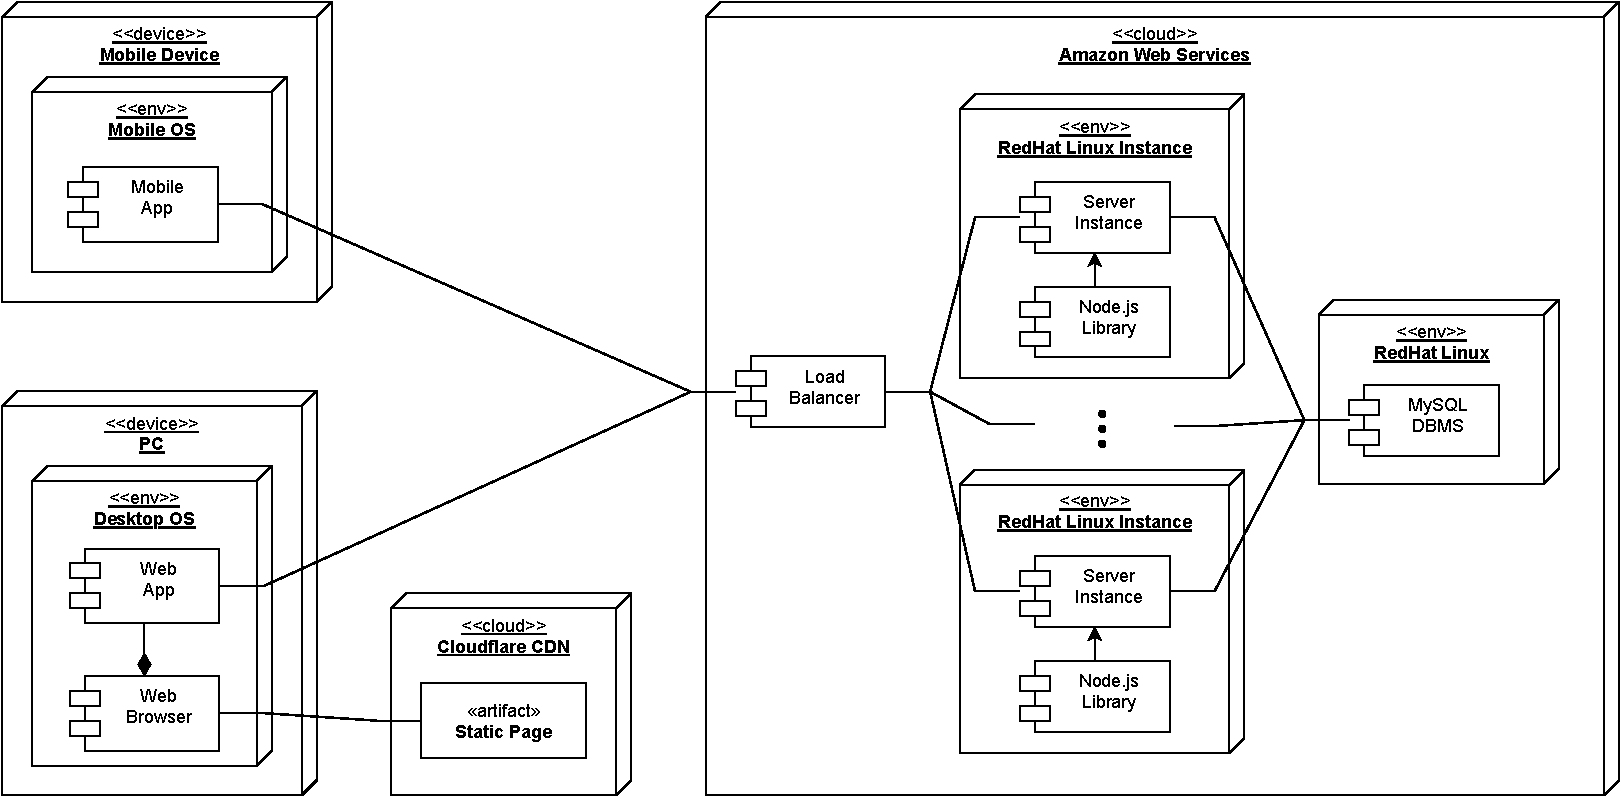
\includegraphics[width=\linewidth]{images/draw.io/deployment_structure.pdf}
    \caption{Deployment Diagram}
    \label{fig:deployment_structure}
\end{figure}

\subsection{Runtime View}
% You can use sequence diagrams to describe the way components interact
% to accomplish specific tasks typically related to your use cases

\begin{figure}[H]
    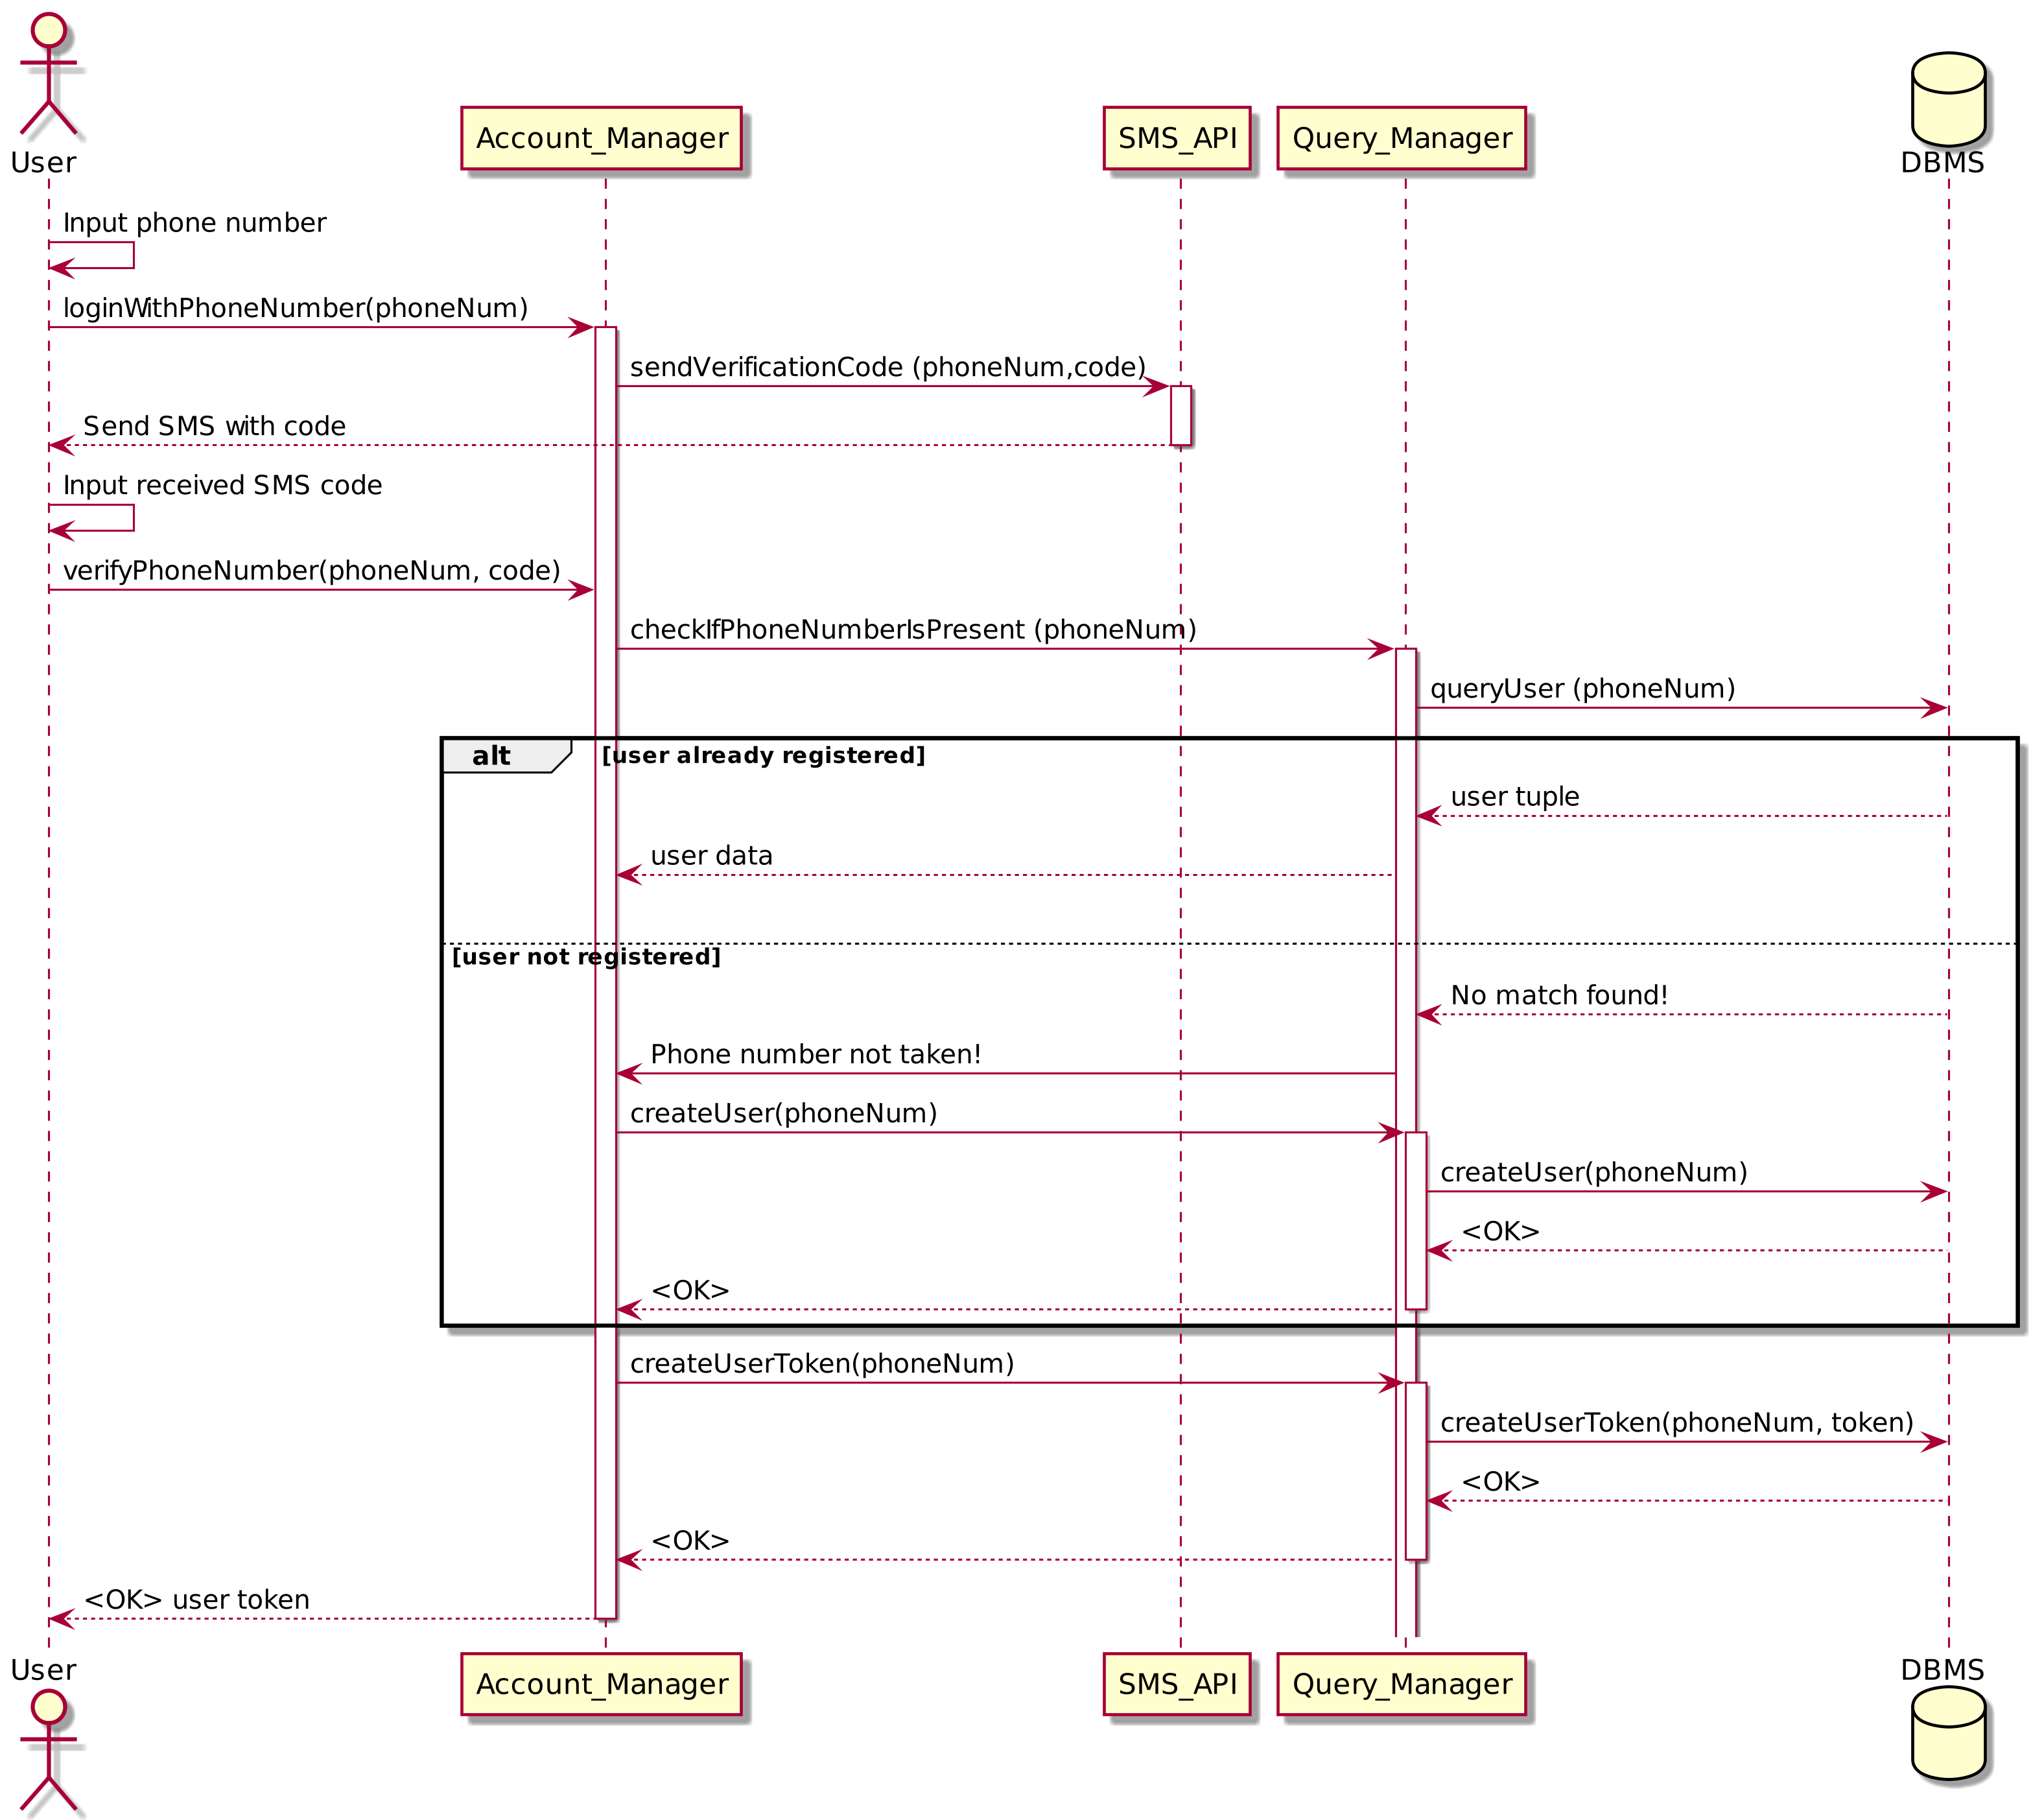
\includegraphics[width=\linewidth]{uml/seq_user_login.png}
    \caption{User Login}
    \label{fig:seq_user_login}
\end{figure}

\begin{figure}[H]
    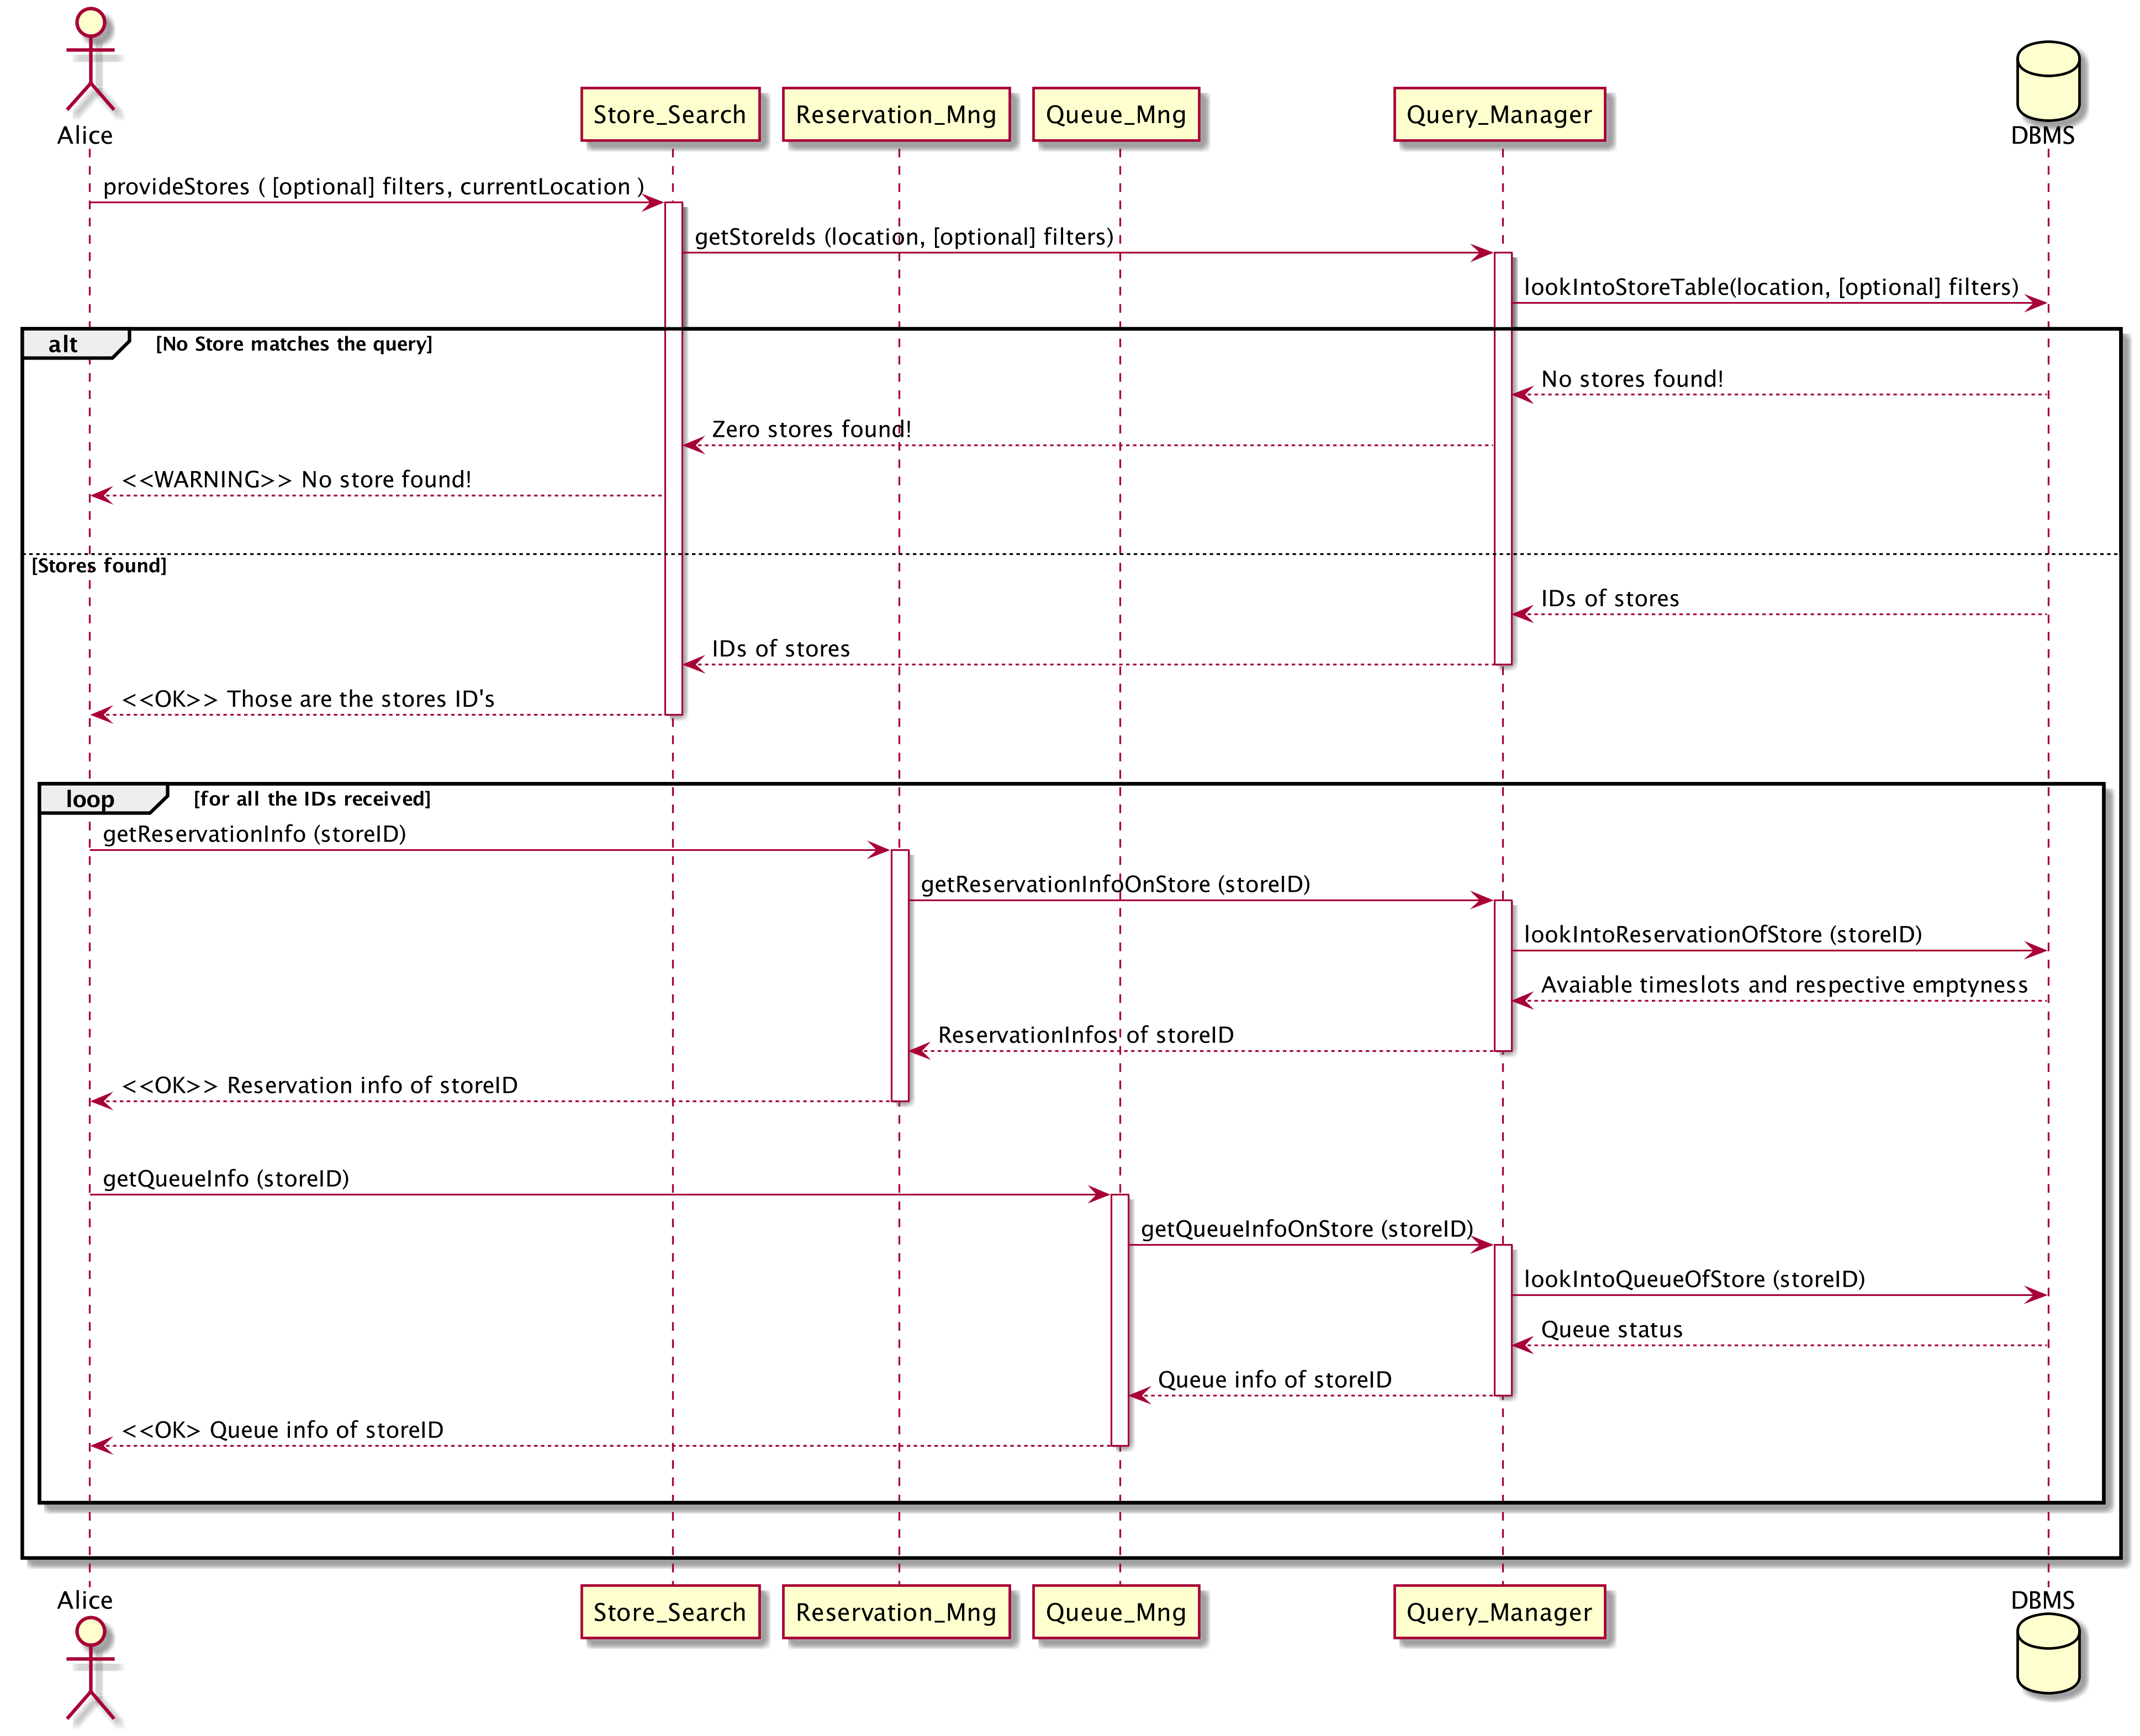
\includegraphics[width=\linewidth]{uml/seq_search_store.png}
    \caption{Store search}
    \label{fig:seq_store_search}
\end{figure}

\begin{figure}[H]
    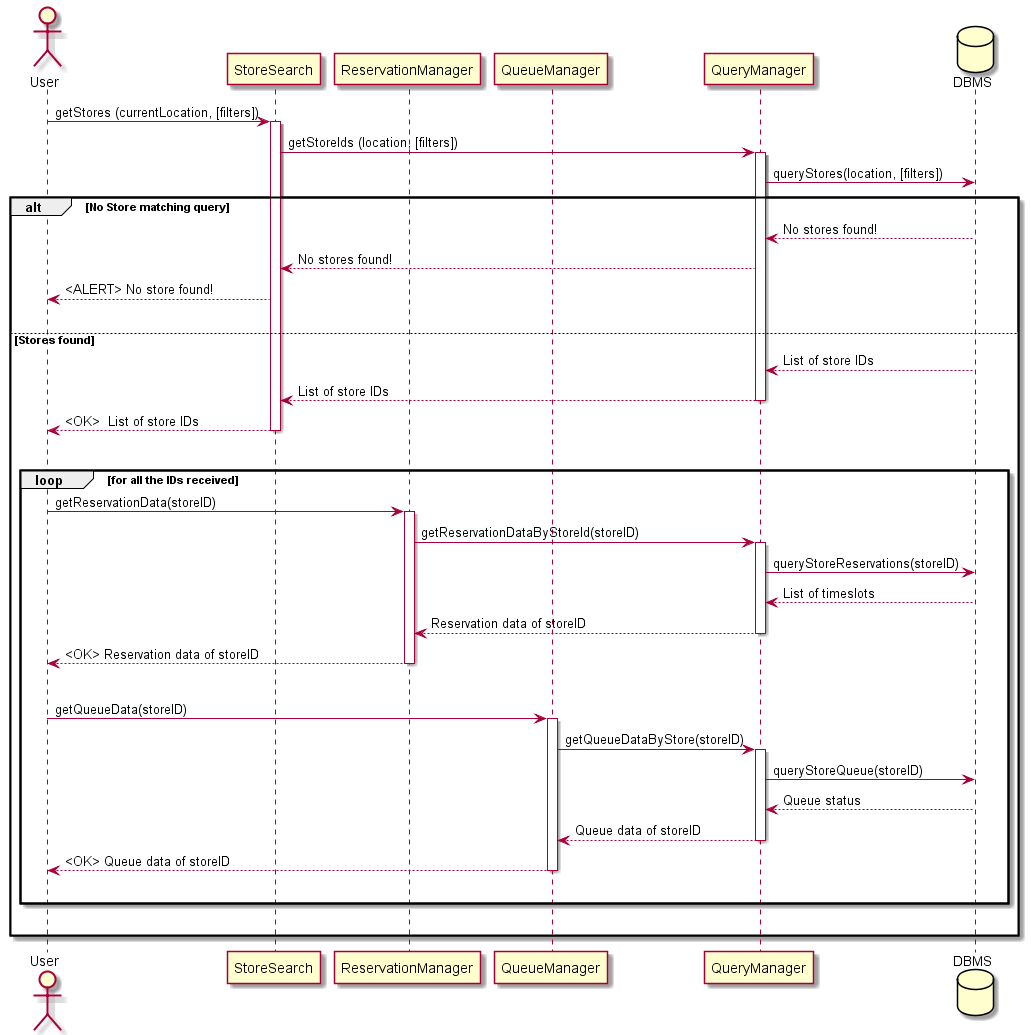
\includegraphics[width=\linewidth]{uml/seq_join_queue.png}
    \caption{User joins queue}
    \label{fig:seq_join_queue}
\end{figure}


\begin{figure}[H]
    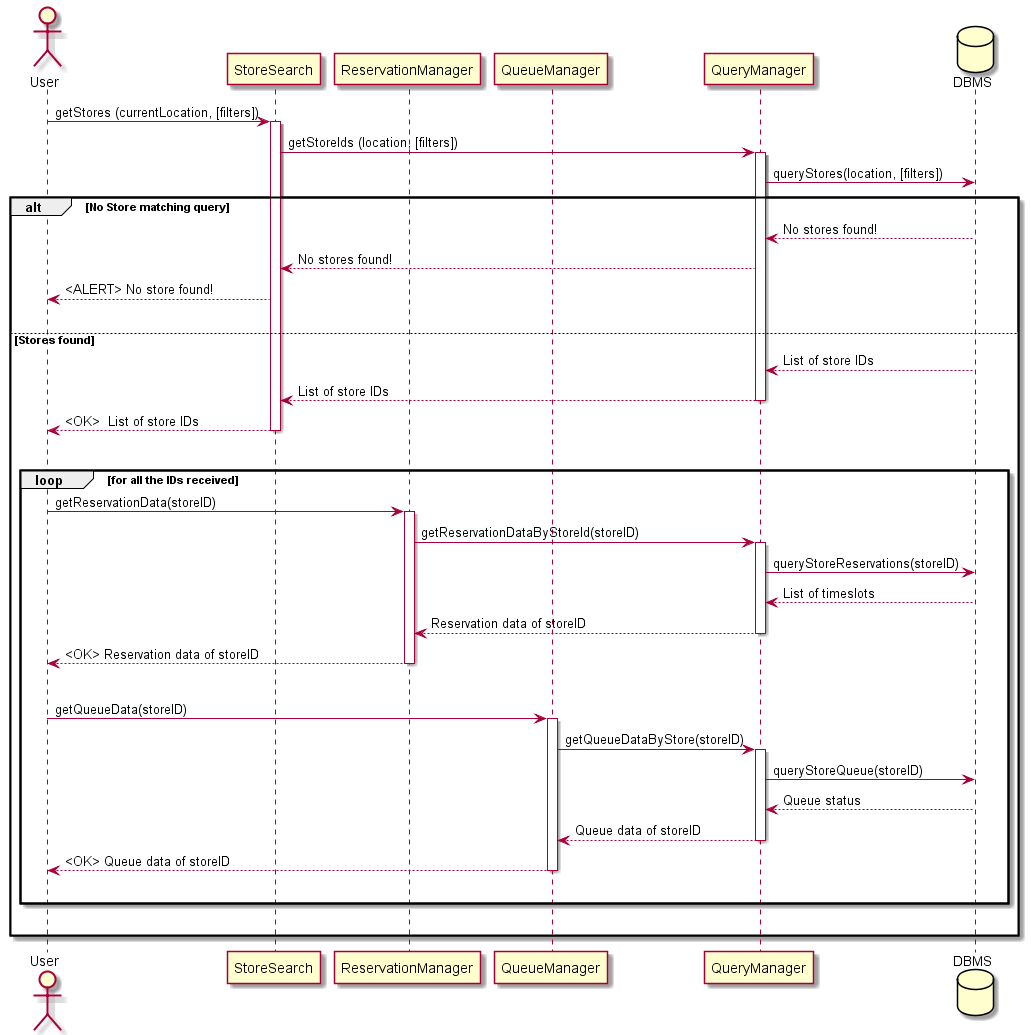
\includegraphics[width=\linewidth]{uml/seq_join_queue.png}
    \caption{User joins queue}
    \label{fig:seq_join_queue}
\end{figure}

\begin{figure}[H]
    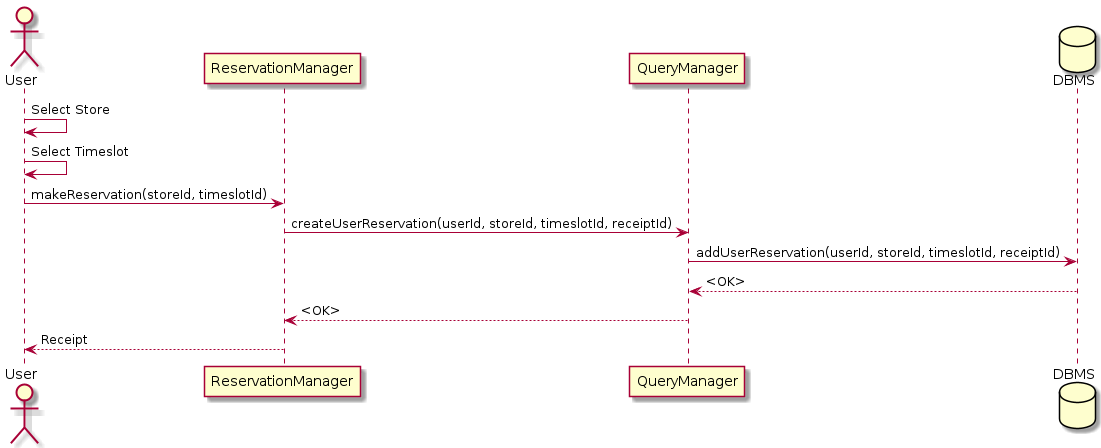
\includegraphics[width=\linewidth]{uml/seq_make_reservation.png}
    \caption{User makes a reservation}
    \label{fig:seq_make_reservation}
\end{figure}

\begin{figure}[H]
    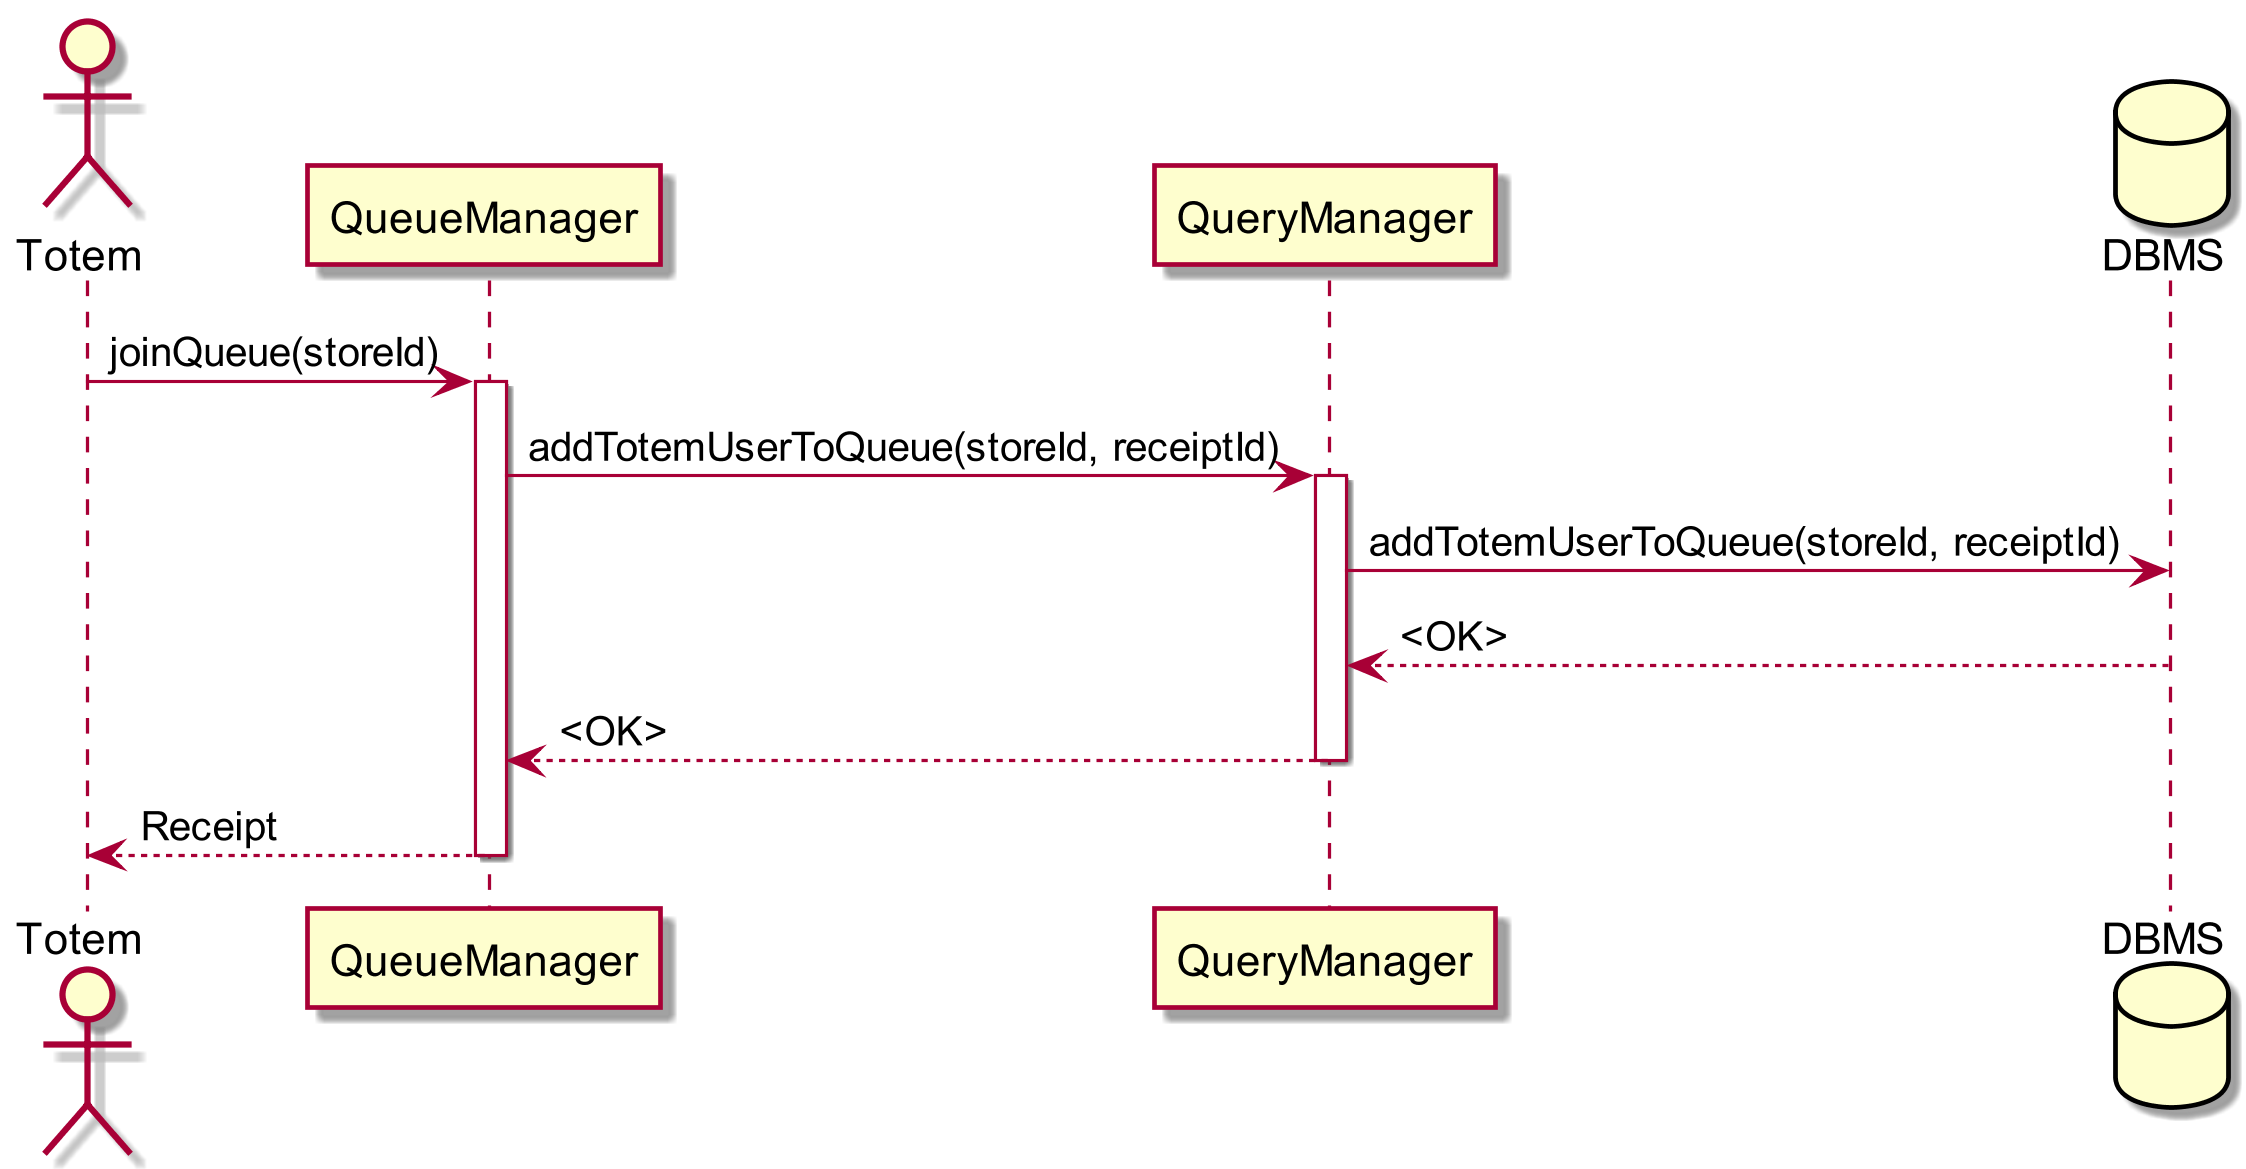
\includegraphics[width=\linewidth]{uml/seq_join_queue_totem.png}
    \caption{User joins the queue from the totem}
    \label{fig:seq_join_queue_totem}
\end{figure}



\subsection{Component Interfaces}

\subsection{Selected Architectural Styles and Patterns}
%  Please explain which styles/patterns you used, why and how
\subsubsection{Architectural Styles}
\paragraph{Thick Client}
The main characteristic of thick clients is offering a wide variety of functionalities independent from the central server.
The main advantages it offers are greater decoupling of frontend and backend and a reduced computational effort on the application server.
Recent years have seen a rise in the adoption of single-page applications, with the advent of cross-platform frameworks which allow to write code that can be run both in an app and in a browser.
This allows developers to reuse significant portions of the codebase across a large number of target platforms, reducing the effort of keeping updated different versions of the same product.
The single-page web application will be served by a dedicated static webserver, which is isolated from the rest of the system.

\paragraph{REST API}
REST is an architectural style centered around the definition of a uniform and predefined set of stateless operations defined on top of the HTTP protocol.
Its main advantages are simplicity, scalability and modifiability.
It allows to have a single endpoint against which both the mobile application and the web application can make requests, therefore eliminating the need of having multiple interfaces, while making it easier to maintain.

\paragraph{Three layer architecture}
Separating presentation, business, and data layers offers great flexibility, maintainability and scalability.
This combined with a thick client means that the only communication between the client and the server goes through a predefined API, without having to worry about eachother's internal representation.

\subsubsection{Patterns}

\paragraph{MVC} The software will be based on the \emph{Model-View-Controller architecture}, where the model resides on the server, and the view on the client. A portion of logic is handled by the client to alleviate load on the server, for example filtering map results. The business logic is manager by the server.

\paragraph{Facade}
All services will be exposed in a reduced minimal API, hiding the real complexity of the system and making available only high level operations to the client.

\paragraph{Adapter}
The Query Manager component implements the Adapter pattern, as it mediates between the business logic and the DBMS services, exposing only a restricted and higher level set of functionalities.

\subsection{Other Design Decisions}

\paragraph{Maps}
The store search screen in the client applications will show the stores on a map for easier navigation and to show a clear view of all possibilities to the user. The maps will be offered by an external service capable of recognizing the addresses of the stores.

\paragraph{SMS}
During the creation of an account the user will be asked to insert their mobile phone number into the system. Then, the user will receive a confirmation code through an SMS sent via an external service, in order to certify their identity. This step is needed in order to mitigate the problem of the creation of fake accounts and fake reservations, which could be used by hacker in order to clog up the system and damage both stores and users.
